\section{Model}
\label{sec:model}

In this section we first formally define snapshot graphs, and then
show how graph evolution is represented by assigning temporal meaning
to sequences of snapshot graphs.

\begin{definition}[Snapshot]
A {\em snapshot graph} (or a {\em snapshot}) is a pair $G = (V,E)$,
where $V$ is a finite set of nodes with schema $(\underline{vid},
a_1, \ldots, a_n)$, and $E$ is a finite set of edges connecting
pairs of nodes from $V$, with schema $(\underline{vid_1},
\underline{vid_2}, a_1, \ldots, a_m)$.
\label{def:sg} 
\end{definition}

\eat{
\begin{figure}
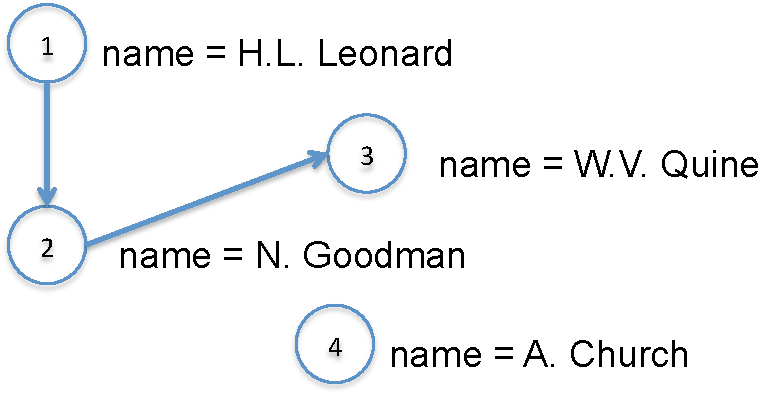
\includegraphics[width=3.2in]{figs/snapshot.pdf}
\caption{Snapshot of DBLP co-authorship graph for 1940, with a single
  string node attribute $name$ and no edge attributes.}
\label{fig:sg}
\end{figure}
}

Attributes of vertices and of edges are not restricted to be of atomic
types, but may, e.g., be maps or tuples. However it is required that
all vertices (resp. edges) of $G$ have the same schema, i.e., $V$ and
$E$ are homogeneous sets.

\begin{definition} [Structural union-compatibility]
Snapshot graphs $G' = (V', E')$ and $G'' = (V'', E'')$ are
union-compatible if $V'$ and $V''$ are union-compatible, and $E'$ and
$E''$ are union-compatible.
\label{def:scompat}
\end{definition}

This is the standard union compatibility definition, which requires
that vertex schema $V$ and edge schema $E$ be the same for $G'$ and
$G''$.\eat{  For example, the snapshot in Figure~\ref{fig:sg} is only
compatible with other snapshots where vertices have one non-key string
attribute $name$ and no non-key edge attributes.}
%
$G$ may represent a directed or an undirected graph.  For undirected
graphs we choose a canonical representation of an edge, with $vid_1
\leq vid_2$ (self-loops are allowed).

We next describe how time is represented in our model.  Following the
SQL:2011 standard~\cite{DBLP:journals/sigmod/KulkarniM12}, we adopt
the {\em closed-open} period model, where a period represents all
times starting from and including the start time, continuing to but
excluding the end time.

\begin{definition}[Time period]
A {\em time period} \\$p = [start, end)$ is an interval on the
  timeline, subject to the constraint $start < end$.  We refer to the
  length of time covered by $p$ as its {\em resolution}, which is
  explicitly associated with a {\em unit of time}.
\label{def:period} 
\end{definition}

Examples of time periods are $p_1=[\tpy{2000},\tpy{2001})$ (a 1-year
  period), $p_2=[\tpym{2000}{12},\tpym{2001}{03})$ (a 3-month period)
    and $p_2=[\tpymd{2000}{12}{01},\tpymd{2001}{03}{01})$ (a 90-day
      period).  The unit of time is application-dependent, and will be
      stated explicitly where not clear from context.

Our goal in this work is to support complex analytics over evolving
graphs, under the assumption that all historical data is available in
the database and is read-only.  For this reason we focus on {\em valid
  time}, represented by {\em application-time period} in SQL:2011 ---
the time period during which data is regarded as correctly reflecting
reality.  This is in contrast to {\em transaction time} (or {\em
  system-time period}), which refers to the time period during which a
row is committed to the database.

We represent graph evolution by associating a sequence of snapshots
(Def.~\ref{def:sg}), which are not themselves time-aware, with a
sequence of time periods.  We now formally define temporal sequences.

\begin{definition} [Temporal Sequence]
A {\em temporal sequence} $P = (p_1, \ldots, p_n)$ is a
sequence of consecutive non-overlapping time periods of the same
resolution, with no gaps.  That is,

\begin{enumerate}
\item $\forall i < n, p_i.end = p_{i+1}.start$, and 
\item $\forall i, j, p_i.end - p_i.start = p_j.end - p_j.start$.
\end{enumerate}
\label{def:tseq} 
\end{definition}

$P$ may be equivalently described by any 2 of the following 3 values:
the start of the earliest period $P.start = p_1.start$, the end of the
latest period $P.end = p_n.end$, and the resolution of any period
$P.res = p_1.end - p_1.start$, specified in appropriate time
units. For convenience, we refer to the number of periods in the
sequence as $P.size$.

For example, $P=([\tpy{1940},\tpy{1945}), \ldots,
  [\tpy{2010},\tpy{2015}))$ represents a temporal sequence with
    $P.start=\tpy{1940}$, $P.end=\tpy{2015}$, $P.res=5$ years, and
    $P.size=15$.

A special sequence $P^{\epsilon}$ is the null sequence, with
$P^{\epsilon}.res=null$, $P^{\epsilon}.start=null$,
$P^{\epsilon}.end=null$, and  $P^{\epsilon}.size=0$.

\eat{\vera{According to the wiki, $[a,a)$ is considered an empty
      set. So if we just follow the standard interval math semantics,
      we can say: A null temporal sequence is a sequence represented
      by the $[p.start,p.end)$ time interval regardless of the
        resolution. By definition it is of size 0.}}

We next define union-compatibility for temporal sequences, and present
two basic operations on temporal sequences.

\begin{definition} [Temporal Union-Compatibility]
Temporal sequences $P'$ and $P''$ are union-compatible if they have
the same resolution, and if we can construct a valid temporal sequence
$P$ with $P.start = min(P'.start, P''.start)$, $P.end = max(P'.end,
P''.end)$, and $P.res = P'.res$.  $P^{\epsilon}$ is union-compatible
with any temporal sequence.
\label{def:tcompat} 
\end{definition}

\begin{example}
Consider the following temporal sequences, with year as the unit of
time.
\begin{itemize}
\item $P_1=([\tpy{2001},\tpy{2003}),[\tpy{2003},\tpy{2005}))$
\item $P_2=([\tpy{2009},\tpy{2010}),[\tpy{2010},\tpy{2011}))$
\item $P_3=([\tpy{2008},\tpy{2010}),[\tpy{2010},\tpy{2012}),[\tpy{2012},\tpy{2014}))$
\item $P_4=([\tpy{2012},\tpy{2014}),[\tpy{2014},\tpy{2016}))$
\item $P_5=([\tpy{2020},\tpy{2022}))$
\end{itemize}

$P_1$ and $P_2$ are not union-compatible because $P_1.res=2 years$,
while $P_2.res = 1 year$.  $P_1$ and $P_3$ are not union-compatible
because, while $P_1.res = P_3.res = 2 years$, it is not possible to
construct a valid temporal sequence with $P.start=\tpy{2001}$,
$P.end=\tpy{2014}$ and $P.res=2 years$.  Finally, $P_3$, $P_4$ and
$P_5$ are pair-wise union-compatible.  
\label{ex:ex1}
\end{example}

As our example illustrates, a pair of union-compatible sequences may
or may not overlap, and may not even be consecutive.

\begin{definition} [Temporal Intersection] 
Intersection of union-compatible sequences $P'$ and $P''$, denoted $P'
\cap P''$, is a sequence $P$, containing intervals that are in common
to $P'$ and $P''$.  If no intervals are in common to $P'$ and $P''$,
this operation returns $P^{\epsilon}$.
\label{def:tseqand}
\end{definition}

Continuing with Example~\ref{ex:ex1}, $P_3 \cap P_4 =
([\tpy{2012},\tpy{2014}))$ and $P_3 \cap P_5 = P^{\epsilon}$.

\begin{definition} [Temporal Union]
Temporal union of union-compatible sequences $P'$ and $P''$, denoted
$P' \cup P''$, is the sequence $P$ with $P.start = min(P'.start,
P''.start)$, $P.end = max(P'.end, P''.end)$, and $P.res = P'.res$.
\label{def:tseqor}
\end{definition}

In Example~\ref{ex:ex1}, $P_3 \cup P_4 =
([\tpy{2008},\tpy{2010}),\ldots,[\tpy{2014},\tpy{2016}))$ and $P_3
    \cup P_5 = ([\tpy{2008},\tpy{2010}), \ldots,
      [\tpy{2020},\tpy{2022}))$.

Recall that a snapshot represents a single state of an evolving graph,
and is not itself time-aware.  Temporal evolution of a graph is
represented by a sequence of snapshots, called {\em temporal graphs}
in our formalism.

\begin{figure}
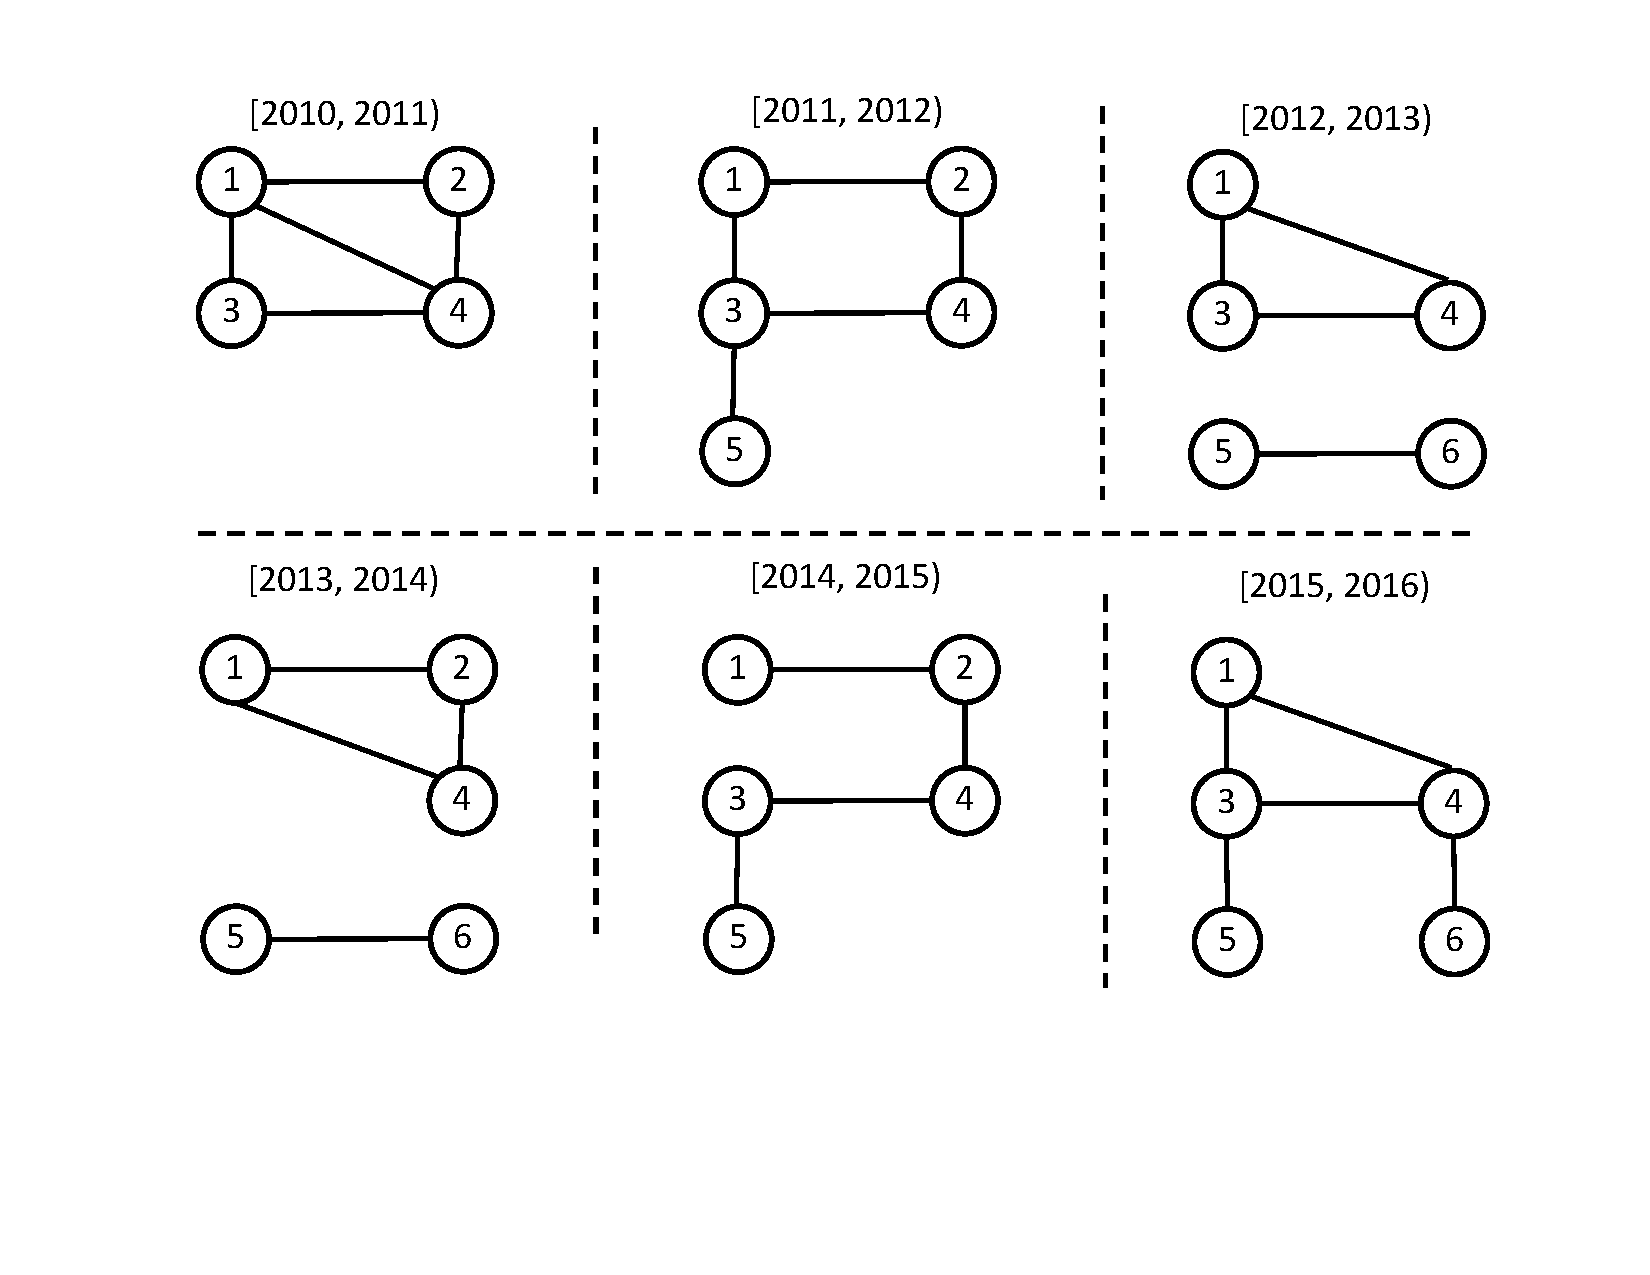
\includegraphics[width=3.2in]{figs/6snaps.pdf}
\caption{\tg \insql{T} with 6 snapshots.} 
\label{fig:tg}
\end{figure}

\begin{figure}
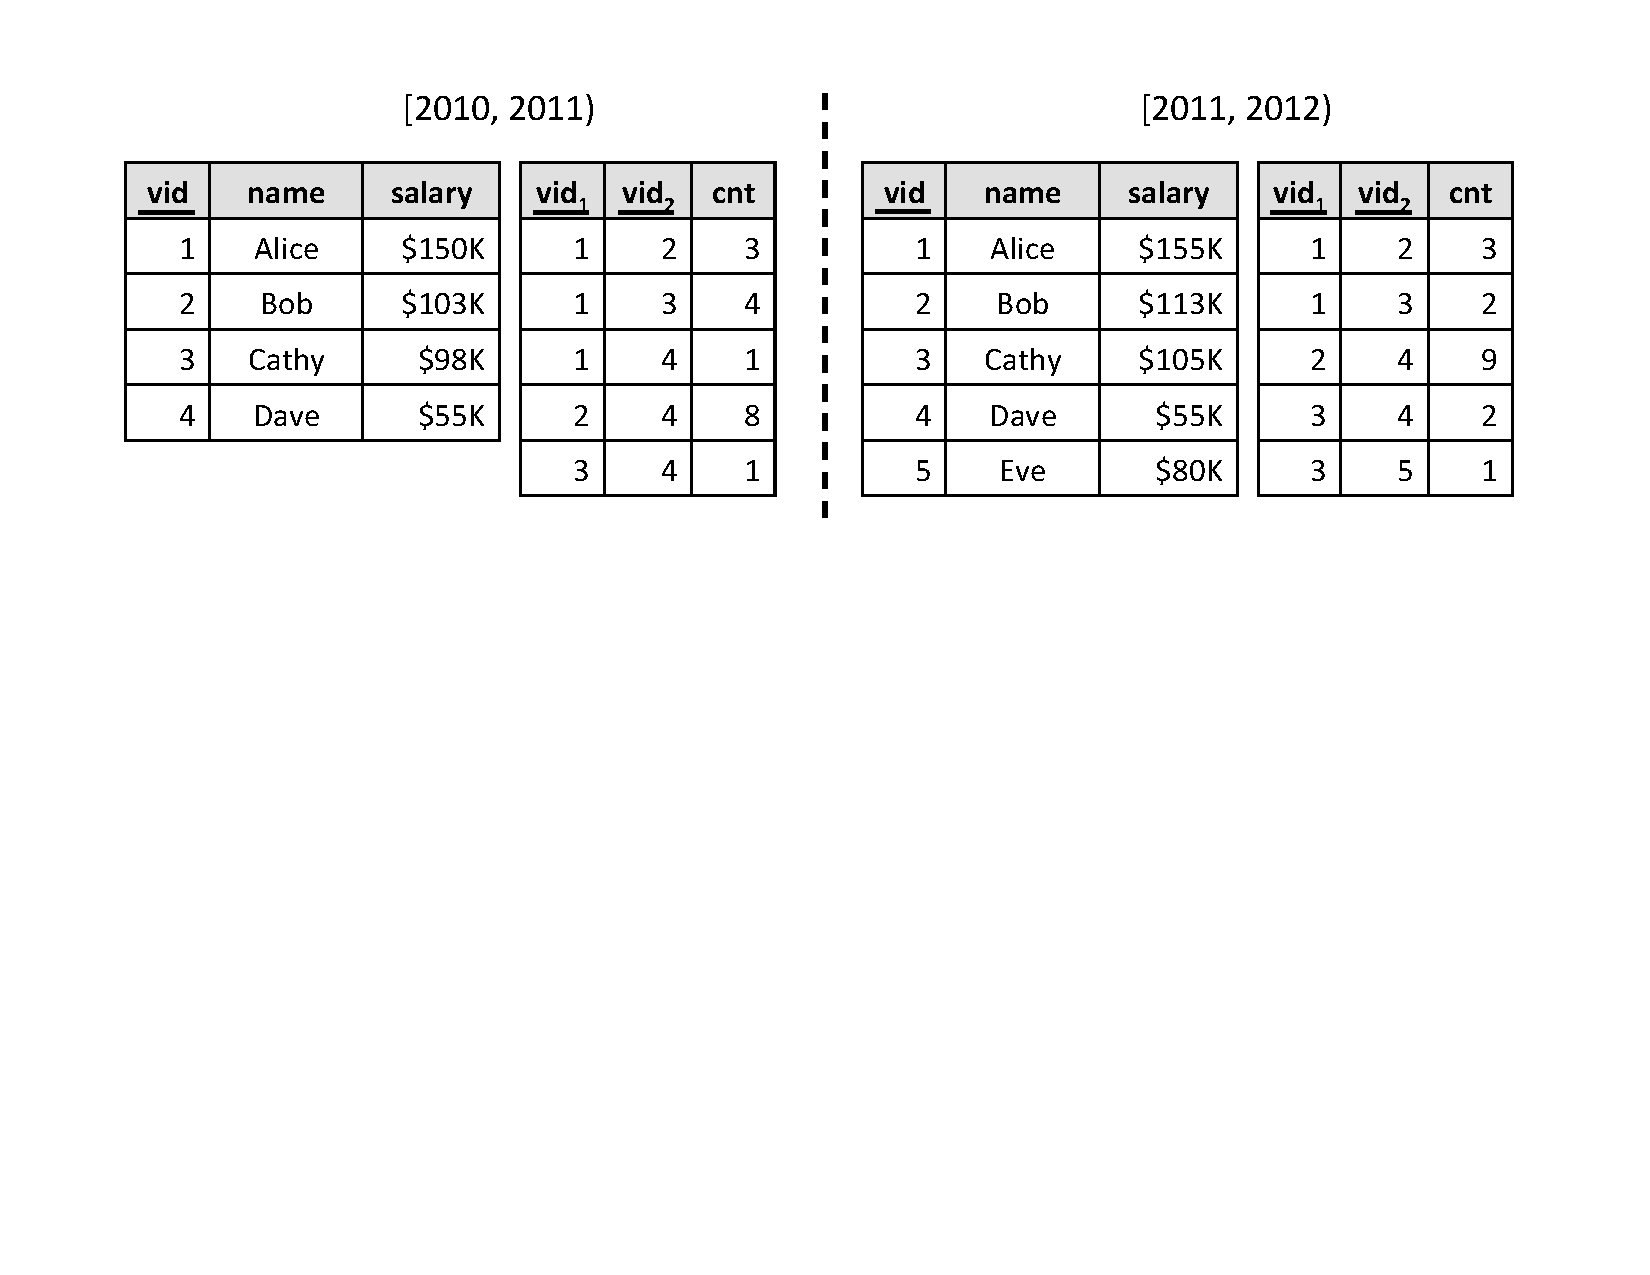
\includegraphics[width=3.5in]{figs/2VE.pdf}
\caption{Vertices and edges of 2 snapshots of \insql{T}.}
\label{fig:2ve}
\end{figure}

\begin{definition} [TGraph]
A {\em temporal graph} (or a {\em \tg}) $T = (G_1, \ldots, G_n; P)$
  associates a sequence of $n$ structurally union-compatible snapshots
  with a temporal sequence $P$, such that $P.size = n$.
\label{def:tgraph} 
\end{definition}

Snapshot graphs in the sequence define the {\em structural schema} of
$T$, while $P$ specifies the {\em temporal schema} of $T$.  

An example of a \tg is given in Figure~\ref{fig:tg}.  Importantly,
identity of a vertex persists across snapshots in a \tg, and across
\tgs.  For example, vertex with id $3$ represents the same entity in
all snapshots in Figure~\ref{fig:tg} in which it occurs.

\eat{
\begin{figure}
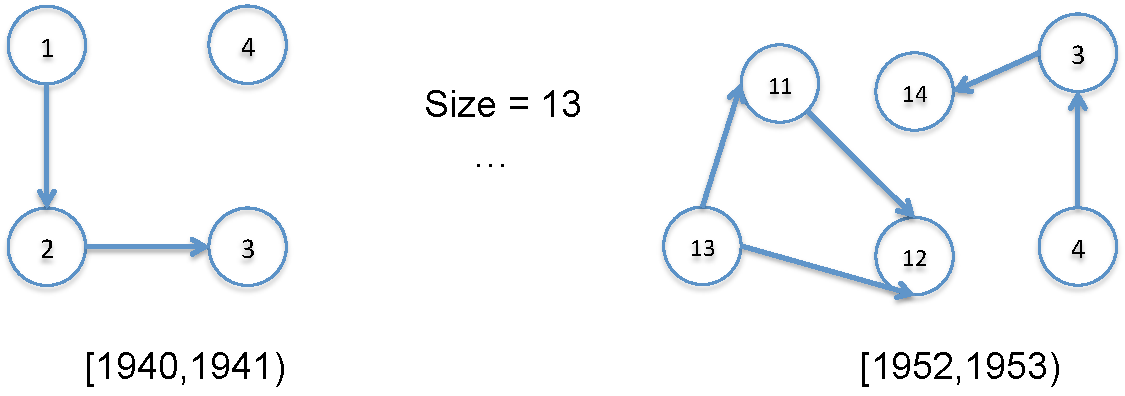
\includegraphics[width=3.2in]{figs/temporalgraph.pdf}
\caption{A \tg of VLDB co-authorship over the period from \tpy{1940} to \tpy{1953}.}
\label{fig:tgraph}
\end{figure}
}

To conclude this section, we define union-compatibility for \tgs.

\begin{definition} [\tg Union-Compatibility]
\label{def:tuc} 
$T'$ and $T''$ are union-compatible \tgs if they are both structurally
union-compatible (per Definition~\ref{def:scompat}) and temporally
union-compatible (per Definition~\ref{def:tcompat}).
\end{definition}

The \tg of Definition~\ref{def:tgraph} is the basic element in our
model.  In what follows, we assume that a relation in our database
corresponds to a single \tg, not to a collection of \tgs.  In the next
section we will present the \ql query langauge that operates on \tgs.




